\section{From RNN to LSTM}

\mode<presentation>{
\begin{frame} 
    \begin{center} \huge
        \secname
    \end{center}
    
    \begin{center}
        RNNs with memory cells\\
        
    Another solution to the vanishing gradient problem in RNNs
    \end{center}
    
    \begin{center}
		
\includegraphics[width=0.2\textwidth]{img/meme_from_rnn_to_lstm}
    \end{center}
    
\end{frame}
}

\definecolor{darkgreen}{rgb}{0,0.5,0}
\definecolor{darkyellow}{rgb}{0.5,0.5,0}
\definecolor{midgreen}{rgb}{0,0.75,0}

\begin{frame}\frametitle{What is an LSTM?}
The long short-term memory (LSTM) cell is an extension of the basic RNN
architecture with memory state cells.
\end{frame}

\begin{frame}\frametitle{The simple RNN unrolled in time}

\mode<presentation>{
\begin{textblock}{}(14.5,2.5)
	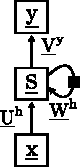
\includegraphics[height=2cm]{img/rnn_superscript}
\end{textblock}
}
    
\begin{center}
	\includegraphics<1>[width=0.8\textwidth]{img/lstm_delay_unroll_simple}
	\notesonly{
	\captionof{figure}{We start constructing our LSTM from a simple RNN unrolled in time.}
	}
\end{center}

\mode<presentation>{
\begin{eqnarray}
		\vec y^{(t)} &=& f\Big( \vec V^\mathrm{y} \, \vec s^{(t)} + \vec b^\mathrm{y}
					\Big) \,,
					\qquad \text{e.g.}\;f(\cdot)=\text{softmax}(\cdot) \\[-1mm]
		\vec s^{(t)} &=& \tanh\Big( \vec U^\mathrm{h} \, \vec x^{(t)}  
				+ \vec W^\mathrm{h} \, \vec s^{(t-1)} + \vec b^\mathrm{s}
				\Big)
	\end{eqnarray}	
}

\end{frame}


\begin{frame}
\only<1>{\frametitle{Simple RNN + memory state cells}}
%\only<2,3,4>{\frametitle{Simple RNN + memory state cells + input gates}}
%\only<5->{\frametitle{Simple RNN + memory state cells + input gates + output gates}}
   
\only<1>{
\begin{center}
	\includegraphics<1>[width=0.8\textwidth]{img/lstm_delay_unroll_memory_annot}
	\notesonly{
	\captionof{figure}{Adding memory state cells to the simple RNN unrolled in time.}
	}
\end{center}
}
%\only<2,3,4>{
%\begin{center}
%\slidesonly{
	%\includegraphics<2>[width=0.8\textwidth]{img/lstm_delay_unroll_write_gate_only}
	%\includegraphics<3>[width=0.8\textwidth]{img/lstm_delay_unroll_write_connect}
%}
	%\includegraphics<4>[width=0.8\textwidth]{img/lstm_delay_unroll_write}
	%\notesonly{
	%\captionof{figure}{Adding input gates.}
	%}
%\end{center}
%}
%\only<5->{
%\begin{center}
	%\includegraphics<5>[width=0.7\textwidth]{img/lstm_delay_unroll_write_read_gate_only}
	%\includegraphics<6->[width=0.7\textwidth]{img/lstm_delay_unroll_write_read}
	%\notesonly{
	%\captionof{figure}{Adding input and output gates.}
	%}
%\end{center}
%}

\mode<presentation>{
	\svspace{-5mm}
	\begin{eqnarray*}
		\vec c^{(t)} &=& {\color{magenta}1.0}~\vec c^{(t-1)} 
				+  {\color{blue} 
				%\visible<2->{ \vec g^{\mathrm{i}(t)} \odot} 
				 \tanh\Big( 
					\vec W^\mathrm{c} \vec s^{(t-1)} \Big)
					 } \\[-1mm]
		\vec y^{(t)} &=& f\Big( \vec V^\mathrm{y} \, \vec s^{(t)} + \vec b^\mathrm{y}
					+ {\color{darkgreen} \vec U^\mathrm{y} 
					%\visible<6->{\big(} 
					\vec c^{(t)} 
					%\visible<5->{\odot \vec g^{\mathrm{o}(t)} \big)}
					 } 
					\Big) \,,
					\qquad \text{e.g.}\;f(\cdot)=\text{softmax}(\cdot) \\[-1mm]
		\vec s^{(t)} &=& \tanh\Big( \vec U^\mathrm{h} \, \vec x^{(t)}  
				+ \vec W^\mathrm{h} \, \vec s^{(t-1)} + \vec b^\mathrm{s}
				+ {\color{darkgreen} \vec V^\mathrm{h} 
					%\visible<6->{\big(} 
					\vec c^{(t-1)} 
					%\visible<5->{\odot \vec g^{\mathrm{o}(t)} \big)} 
					}
				\Big) \\[-1mm]
		%\visible<2->{\color{blue} \vec g^{\mathrm{i}(t)}} 
			%&\visible<2->{\color{blue}=}& 
			%\visible<3->{\color{blue}
				%\sigma\Big(\vec U^\mathrm{i} \, \vec x^{(t)} 
				%+ \vec V^\mathrm{i} \, \vec c^{(t-1)} 
				%+ \vec W^\mathrm{i} \, \vec s^{(t-1)} 
				%+ \vec b^\mathrm{i} \Big) } \\[-1mm]
		%\visible<5->{\color{darkgreen} \vec g^{\mathrm{o}(t)}} 
			%&\visible<5->{\color{darkgreen}=}& 
			%\visible<6->{\color{darkgreen}
				%\sigma\Big(\vec U^\mathrm{o} \, \vec x^{(t)} 
				%+ \vec V^\mathrm{o} \, \vec c^{(t-1)} 
				%+ \vec W^\mathrm{o} \, \vec s^{(t-1)} 
				%+ \vec b^\mathrm{o} \Big) } 
	\end{eqnarray*}	
	}

\end{frame}

%\begin{frame}{Building an LSTM from an RNN}

%\mode<presentation>{
%\begin{center}
	%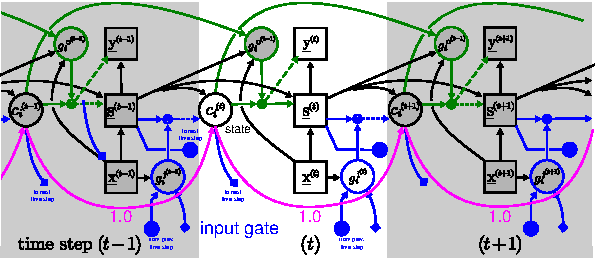
\includegraphics[width=0.7\textwidth]{img/lstm_delay_unroll_write_read}
%\end{center}

%\pause

%\begin{center}
	%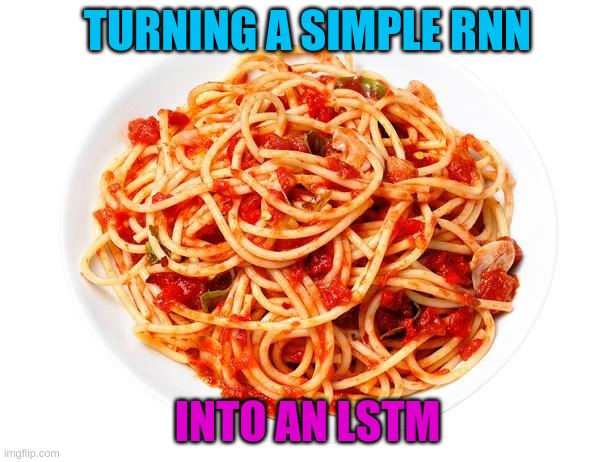
\includegraphics[width=0.4\textwidth]{img/meme_lstm_spaghetti}
%\end{center}
%}
%\end{frame}

\begin{frame}{Building an LSTM from an RNN}



\mode<presentation>{
\only<1>{
\begin{center}
	\includegraphics<1>[width=0.8\textwidth]{img/lstm_delay_unroll_memory_annot}
\end{center}
}

\mode<presentation>{
	%\begin{textblock}{}(10.25,2.5)
\begin{center}
		\includegraphics<1>[height=3cm]{img/lstm_feedback_delay}
\end{center}
	%\end{textblock}
    }
}
\end{frame}

\clearpage

% ------------------------------------------------------------------------------
\begin{frame}\frametitle{Long short-term memory (LSTM) architecture}
    \mode<presentation>{
	\begin{textblock}{}(10.25,2.5)
		%\includegraphics<1>[height=3cm]{img/lstm_feedback.pdf}
		\includegraphics<1>[height=3cm]{img/lstm_feedback_delay.pdf}
		%\includegraphics<2>[height=3cm]{img/lstm_write.pdf}
		\includegraphics<2>[height=3cm]{img/lstm_write_delay.pdf}
		%\includegraphics<3->[height=3cm]{img/lstm.pdf}
		\includegraphics<3->[height=3cm]{img/lstm_delay_indices.pdf}
	\end{textblock}
    }
    \mode<article>{
	\begin{textblock}{}(10.25,2.5)
		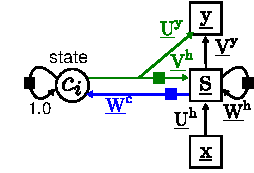
\includegraphics[height=3cm]{img/lstm_feedback_delay.pdf}\\
        
		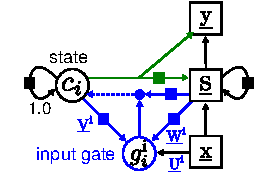
\includegraphics[height=3cm]{img/lstm_write_delay.pdf}\\
        
		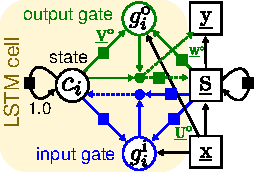
\includegraphics[height=3cm]{img/lstm_delay_indices.pdf}
	\end{textblock}
    }
	
	\begin{textblock}{10}(0.4,2.5)
		\only<1>{ \small
			\iitem{extend the simple RNN with state nodes $\vec c$}
			\vspace{-5mm}
			\iitem{leaky unit $c_i$ with $\alpha_i=1$}
			\vspace{-5mm}
			\iitem{{\color{darkgreen}time delayed feedback} to hidden layer}
			\vspace{-5mm}
			\iitem{{\color{blue} time delayed storage} into state layer 
					%$\sigma(x) = \big( 1 + e^{-x} \big)^{-1}$
					}
		} \only<2>{ \small
			\iitem{introducing an {\color{blue}input (``write'') gate 
					$g_i^\mathrm{i}$}
					\vspace{-2mm}
					\iitem{\footnotesize gate transfer function
							$\sigma(x) = \big( 1 + e^{-x} \big)^{-1}$} }
			\vspace{-4mm}
			\iitem{state input is multiplied ($\color{blue}\otimes$) with gate}
			\vspace{-5mm}
			\iitem{state $c_i$ only changes when 
					{\color{blue}$g_i^{\mathrm{i}(t)} \gg 0$}}
			\vspace{-5mm}
			%\iitem{local errors $\delta_i^{(t)}$ still accumulate in $c_i$}
		} \only<3>{ \small
			\iitem{introducing an {\color{darkgreen}output 
					(``read'') gate $g_i^\mathrm{o}$}
					\vspace{-2mm}
					\iitem{\footnotesize gate transfer function
							$\sigma(x) = \big( 1 + e^{-x} \big)^{-1}$} }
			\vspace{-4mm}
			\iitem{state output is multiplied 
					($\color{darkgreen}\otimes$) with gate}
			\vspace{-5mm}
			\iitem{error $\delta_i^{(t)}$ only changes when 
					{\color{darkgreen}$g_i^{\mathrm{o}(t)} \gg 0$}}
			\vspace{-4mm}
			\iitem{both gates and the state form an {\color{darkyellow}LSTM cell}}
		} \only<4>{ \small\vspace{-1mm}
			\iitem{gates determine access to the state $c_i$
				\vspace{-1mm}
				\iitem{$\color{blue}g_i^{\mathrm{i}}$  learns 
					what to remember}
				\vspace{-3mm}
				\iitem{$\color{darkgreen}g_i^\mathrm{o}$ 
					learns when use the memory} }
			\vspace{-4mm}
			\iitem{gates regulate the flow of activity and error
				\vspace{-1mm}
				\iitem{$\color{blue}g_i^{\mathrm{i}}$ regulates 
						the forward-pass}
				\vspace{-3mm}
				\iitem{$\color{darkgreen}g_i^\mathrm{o}$ 
					regulates the backward-pass} }
		}
	\end{textblock}
	
	\begin{textblock}{10}(0.8,7.5)
	\small
	\begin{eqnarray*}
		\vec c^{(t)} &=& \vec  c^{(t-1)} 
				+  {\color{blue} \visible<2->{ \vec g^{\mathrm{i}(t)} \odot}  \tanh\Big( 
					\vec W^\mathrm{c} \vec s^{(t-1)} \Big)
					 } \\[-1mm]
		\vec y^{(t)} &=& f\Big( \vec V^\mathrm{y} \, \vec s^{(t)} + \vec b^\mathrm{y}
					+ {\color{darkgreen} \vec U^\mathrm{y} 
					\visible<3->{\big(} \vec c^{(t)} 
					\visible<3->{\odot \vec g^{\mathrm{o}(t)} \big)} } 
					\Big) \,,
					\qquad \text{e.g.}\;f(\cdot)=\text{softmax}(\cdot) \\[-1mm]
		\vec s^{(t)} &=& \tanh\Big( \vec U^\mathrm{h} \, \vec x^{(t)}  
				+ \vec W^\mathrm{h} \, \vec s^{(t-1)} + \vec b^\mathrm{s}
				+ {\color{darkgreen} \vec V^\mathrm{h} 
					\visible<3->{\big(} \vec c^{(t-1)} 
					\visible<3->{\odot \vec g^{\mathrm{o}(t)} \big)} }
				\Big) \\[-1mm]
		\visible<2->{\color{blue} \vec g^{\mathrm{i}(t)}} 
			&\visible<2->{\color{blue}=}& 
			\visible<2->{\color{blue}
				\sigma\Big(\vec U^\mathrm{i} \, \vec x^{(t)} 
				+ \vec V^\mathrm{i} \, \vec c^{(t-1)} 
				+ \vec W^\mathrm{i} \, \vec s^{(t-1)} 
				+ \vec b^\mathrm{i} \Big) } \\[-1mm]
		\visible<3->{\color{darkgreen} \vec g^{\mathrm{o}(t)}} 
			&\visible<3->{\color{darkgreen}=}& 
			\visible<3->{\color{darkgreen}
				\sigma\Big(\vec U^\mathrm{o} \, \vec x^{(t)} 
				+ \vec V^\mathrm{o} \, \vec c^{(t-1)} 
				+ \vec W^\mathrm{o} \, \vec s^{(t-1)} 
				+ \vec b^\mathrm{o} \Big) } 
	\end{eqnarray*}	
	
	
	\only<4>{
	\vspace{-5mm}
	
	\question{Why does ${\color{blue}\tanh(\cdot)}$ make sense here?
	}
	
	\notesonly{
	}
	}
	
	\end{textblock}
	
	
	\begin{textblock}{20}(2.75,14.9)
		\footnotesize\only<1-2>{\citep[Section 10.10]{Hochreiter97,Goodfellow16}}
	\end{textblock}
	
	
\end{frame}

\clearpage

\begin{frame}\frametitle{LSTM with forget gate}
\begin{figure}[ht]
     \centering
	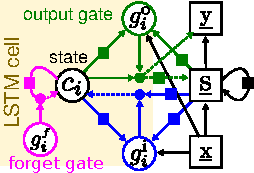
\includegraphics[width=0.4\textwidth]{img/lstm_delay_forget.pdf}
     \mode<article>{
	\caption{Basic RNN architecture}
	}
	\label{fig:rnn} 
\end{figure}
\pause

\begin{equation}
		{\color{magenta} \vec g_i^{\mathrm{f}(t)}} 
			= 
			\color{magenta}
				\sigma\Big(\vec U^\mathrm{f} \, \vec x^{(t)} 
				+ \vec V^\mathrm{f} \, \vec c^{(t-1)} 
				+ \vec W^\mathrm{f} \, \vec s^{(t-1)} 
				+ \vec b^\mathrm{f} \Big) 
\end{equation}

Consequently:
\begin{equation}
		\vec c^{(t)} = {\color{magenta}\vec g^{\mathrm{f}(t)} \odot\,} \vec  c^{(t-1)} 
				+  {\color{blue} { \vec g^{\mathrm{i}(t)} \odot}  \tanh\Big( 
					\vec W^\mathrm{c} \vec s^{(t-1)} \Big)
					 }
\end{equation}


\end{frame}

\subsection{Complexity}

\begin{frame}\frametitle{\subsecname}
\mode<presentation>{
\only<1>{
			\placeimage{13}{1}{img/rnn_superscript}{width=2cm}
			}
\only<2->{
			\placeimage{9}{1}{img/lstm_delay_forget}{width=5cm}
			}
}
		For $\vec x \in \R^N, \vec s \in \R^H, \vec y \in \R^M$:\\
		\begin{itemize}
		\item[]
			Simple RNN:\\
			\begin{itemize}
			\item $\vec U^{\mathrm{h}} \in \R^{H,N},\quad \vec b^{\mathrm{h}} \in \R^{H}$
			\item $\vec W^{\mathrm{h}} \in \R^{H,H}$
			\item $\vec V^{\mathrm{y}} \in \R^{M,H},\quad \vec b^{\mathrm{y}} \in \R^{M}$
			\end{itemize}
			\pause
			
		\item[]
			LSTM:\\
			All of the above in addition to\ldots
			for $\vec c, {\color{blue}\vec g^{\mathrm{i}}}, {\color{darkgreen}\vec g^{\mathrm{o}}}, {\color{magenta}\vec g^{\mathrm{f}}} \in \R^K$\\
			(often $K=H$):\\
			\pause
			\begin{itemize}
			\item for $\vec c$:
             $\color{blue}\vec W^{\mathrm{c}} \in \R^{K,H}$, 
			 $\color{darkgreen}\vec U^{\mathrm{y}} \in \R^{M,K}$,
			 $\color{darkgreen}\vec V^{\mathrm{h}} \in \R^{H,K}$
			\item[] for ${\color{blue}\vec g^{\mathrm{i}}}$:
            \begin{itemize}
                \item $\color{blue}\vec U^{\mathrm{i}} \in \R^{K,N}$
                \item $\color{blue}\vec V^{\mathrm{i}} \in \R^{K,K}$
                \item $\color{blue}\vec W^{\mathrm{i}} \in \R^{K,H}, \quad \vec b^{\mathrm{i}} \in \R^{K}$
			\end{itemize}
            \item duplicate $\color{blue}\vec U^{\mathrm{i}}, \color{blue}\vec V^{\mathrm{i}}, \color{blue}\vec W^{\mathrm{i}}$
			for the output gate $\leadsto \color{darkgreen}\vec U^{\mathrm{o}}, \color{darkgreen}\vec V^{\mathrm{o}}, \color{darkgreen}\vec W^{\mathrm{o}}$ and $\color{darkgreen}\vec b^{\mathrm{o}}$
			\item and for the forget gate $\leadsto \color{magenta}\vec U^{\mathrm{f}}, \color{magenta}\vec V^{\mathrm{f}}, \color{magenta}\vec W^{\mathrm{f}}$ and $\color{magenta}\vec b^{\mathrm{f}}$
			\end{itemize}
		\end{itemize}
		
		\only<4->{
		\slidesonly{
		\placeimage{12}{9.5}{img/meme_lstm_cost}{height=1.7cm}
		}
		}
       
\end{frame}

\begin{frame}\frametitle{\subsecname}

		\question{What about the complexity of echo state networks?}
		
\mode<presentation>{
\begin{center}
	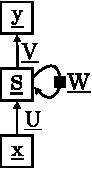
\includegraphics[height=3cm]{img/rnn}
\end{center}
}
		
\pause

%\mode<article>{
        - The hidden-output weights $\vec V$ are the only trainable parameters in echo state networks.
%}


\end{frame}
